\documentclass[a4paper, 12pt, french]{report}
\usepackage[utf8]{inputenc}
\usepackage[french]{babel}
\usepackage[T1]{fontenc}
\usepackage[babel=true]{csquotes}
\usepackage{palatino}
\usepackage{hyperref}
\usepackage{eurosym}
\usepackage{graphicx}
\usepackage{array}
\usepackage{fancyhdr}
\usepackage{lastpage}
\usepackage{xspace}
\usepackage{float}
\usepackage{geometry}
\addtolength{\oddsidemargin}{-.875in}
\addtolength{\evensidemargin}{-.875in}
\addtolength{\textwidth}{1.75in}

\addtolength{\topmargin}{-.5in}
\addtolength{\textheight}{1.75in}
%% -- Commandes personalisées

% Contrainte : chaîne de caractères sans espace, en minuscule, constituée seulement des 26 caractères non accentués de l’alphabet latin
\newcommand{\nomProjet}{enflatme\xspace}
% Contrainte : chaîne de caractères sans espace, en minuscule, constituée seulement des 26 caractères non accentués de l’alphabet latin
\newcommand{\nomEquipe}{teamflat\xspace}

\pagestyle{fancy}
% En-têtes
\renewcommand{\headrulewidth}{1pt}
\fancyhead[C]{\nomProjet} 
\fancyhead[L]{Cahier des charges}
\fancyhead[R]{}

\renewcommand{\footrulewidth}{1pt}
\fancyfoot[C]{Version 1.0} 
\fancyfoot[L]{\nomEquipe\xspace G1}
\fancyfoot[R]{Page \thepage\xspace sur \pageref{LastPage}}

%% -- Document
\begin{document}
	\begin{titlepage}
		\begin{center}
			\LARGE{\bsc{Cahier des charges}} \\
		    \rule{\linewidth}{1.5pt}
		    \huge{\textbf{\nomProjet}}
		    \rule{\linewidth}{1.5pt} \newline{} \newline{}
		\end{center}
		\begin{center}
		    \large{Auteurs :}\\ Antoine \bsc{Augusti} (ANT)\\ Étienne \bsc{Batise} (BAT) \\ Thibaud \bsc{Dauce} (TIB)
		\end{center}
		\vspace{50px}
		\begin{center}
			\large{Date de publication :}\\ \today
		\end{center}
	\end{titlepage}
	\newpage

	% Table des matières
	\tableofcontents
	\pagebreak

	% Début du document
	\chapter{Fondements du projet}
		\section{But du projet}
			\subsection{Problème de l'utilisateur}
Notre objectif est de proposer une application pour simplifier la vie des gens vivant dans une colocation. La vie entre colocataires implique des contraintes et des problèmes ; l'objectif de notre application est de les gérer plus facilement et plus efficacement.

\subsection{Objectifs du projet}
Nous voulons réaliser cette application pour qu'elle s'impose comme un outil incontournable de gestion pour toutes les personnes vivant dans une colocation. Nous voulons leur rendre la vie plus facile en faisant en sorte que les petits tracas de la vie entre colocataires soient fortement réduits.

		\section{Personnes et organismes impliqués dans les enjeux du projet}
			\subsection{Maître d'ouvrage}
Les maîtres d'ouvrage sont :
\begin{itemize}
	\item Antoine Augusti, étudiant à l'Institut National des Sciences Appliquées de Rouen ; 
	\item Étienne Batise, étudiant à l'Institut National des Sciences Appliquées de Rouen ; 
	\item Thibaud Dauce, étudiant à l'Institut National des Sciences Appliquées de Rouen.
\end{itemize}

\subsection{Acheteur}
L'acheteur est la société Teamflat où travaillent les maîtres d'ouvrage cités précédemment.

		\section{Utilisateurs du produit}
			\subsection{Utilisateurs directs du produit}
Les utilisateurs de notre application seront les personnes vivant dans une colocation. La majorité des personnes vivant dans une colocation sont des étudiants puisque ceux-ci ont souvent peu de moyens financiers et choisissent de vivre en colocation pour réaliser des économies.\\

Notre cible est donc un public jeune, entre 18 et 25 ans, autant hommes que femmes. Certains jeunes actifs font également le choix de la colocation. Notre public utilise très fréquemment et maîtrise les dernières nouveautés technologiques et télécharge très régulièrement de nouvelles applications.\\

Concernant les centres d'intérêt de notre cible ils sont autour des sorties, de la musique, des soirées, des jeux-vidéos, des sports\dots Notre cible n'a pas beaucoup de temps à consacrer à la réalisation de tâches ménagères et n'apprécie pas perdre du temps avec ceci. 

\subsection{Priorité assignée aux utilisateurs}
Les utilisateurs sont notre priorité ultime car nous réalisons une application pour répondre à leurs besoins. De plus, nous comptons sur nos utilisateurs pour réaliser la promotion de notre application et ainsi faire en sorte que celle-ci ait une croissance virale.

\subsection{Implication nécessaire de la part des utilisateurs dans le projet}
Aucune implication particulière des utilisateurs n'est nécessaire pour mener à bien le projet. Toutefois, étant donné qu'il est primordial de concevoir un produit qui convient à notre cible que sont les colocataires, il est important de travailler de manière proche avec certains d'entre eux afin d'avoir leur avis sur l'avancement et l'orientation du projet.

\subsection{Utilisateurs concernés par les opérations de maintenance du produit}
Aucun utilisateur ne devra être concerné par des opérations de maintenance car les données devront être stockée sur un des serveurs de la société Teamflat.

	\chapter{Contraintes sur le projet}
		\section{Contraintes non négociables}
			\subsection{Contraintes sur la conception de la solution} % (fold)
\label{sub:contraintes_sur_la_conception_de_la_solution}

	\subsubsection{Téléphone mobile Android}
	L'application doit être utilisable sur un smartphone Android équipé d'une version du système d'exploitation supérieur à la version 4 afin de cibler le maximum d'utilisateurs.

	\subsubsection{Code source}
	Le code source doit répondre à certaines exigences afin d'être libéré sous license libre dans un second temps :\\

	Le code source doit être lisible. Les développeurs ne doivent pas utiliser d'abrévations pour les noms des variables, le camel case doit être privilégié pour le nom de variables et des fonctions. Les développeurs doivent dans la mesure du possible utiliser des opérateurs litéraux (comme 'AND' ou 'OR') à la place d'opérateurs moins lisibles (comme '\&\&' ou '||'). Les développeurs ne doivent en aucun cas utiliser des conditions ternaires. Pour finir, le language de programmation choisi doit permettre une lecture facile.\\

	Le code source doit être commenté de manière efficace. Les commentaires ne doivent pas surcharger le code source mais doivent être présent afin d'expliquer les parties complexes des fonctions. La décomposition d'un problème doit toujours être priviligiée à la surcharge d'une fonction. Les fonctions et les parties de code dites 'simples' et compréhensibles par tous ne doivent pas être commentées. Un code lisible doit toujours être priviligié par rapport à des commentaires.\\

	Enfin, les fonctions du code source doivent être documentées afin de pouvoir générer une documentation de manière automatique (avec des outils tels que Doxygen ou JavaDoc par exemple). Chaque fonction doit présenter une description succinte, le nom des paramètres en entrée et le nom des paramètres en sortie. En cas de complexité plus importante ou d'une incompréhension possible, la documentation doit afficher une description plus complète et/ou une description de chaque attribut en entrée ou en sortie.


% subsection contraintes_sur_la_conception_de_la_solution (end)

\subsection{Environnement de fonctionnement du système actuel} % (fold)
\label{sub:environnement_de_fonctionnement_du_syst_me_actuel}

	Le but du projet est de créer une application à partir de zéro. Aucun système actuel n'est en place.

% subsection environnement_de_fonctionnement_du_syst_me_actuel (end)

\subsection{Applications partenaires} % (fold)
\label{sub:applications_partenaires}

	Nous n'envisageons aucun lien avec des applications tierces. En particulier avec les réseaux sociaux, notre application doit être complètement indépendante.

% subsection applications_partenaires (end)

\subsection{COTS : progiciels ou composants commerciaux} % (fold)
\label{sub:cots_progiciels_ou_composants_commerciaux}

	N/A

% subsection cots_progiciels_ou_composants_commerciaux (end)

\subsection{Lieux de fonctionnement prévus} % (fold)
\label{sub:lieux_de_fonctionnement_pr_vus}

	Le lieu principal de fonctionnement prévu est la collocation. Les personnes seront dans un environnement familier, sans bruit et tranquille. Ils auront à disposition un ordinateur fixe ou portable ainsi qu'un smartphone.

	Malgré la tranquilité du lieu, l'application doit être rapidement exécutable afin d'effectuer les mises à jour de ses activités rapidement.

% subsection lieux_de_fonctionnement_pr_vus (end)

\subsection{De combien de temps les développeurs disposent-ils pour le projet} % (fold)
\label{sub:de_combien_de_temps_les_d_veloppeurs_disposent_ils_pour_le_projet}

	Le projet doit être opérationnel fin août afin de permettre aux nouveaux étudiants de s'inscrire dès le début de leur collocation. Les développeurs disposent donc de 4 mois à compter d'aujourd'hui afin de livrer l'application début août et ainsi nous permettre de mettre en place une communication et une campagne marketing pour le lancement du produit.

% subsection de_combien_de_temps_les_d_veloppeurs_disposent_ils_pour_le_projet (end)

\subsection{Quel est le budget affecté au projet ?} % (fold)
\label{sub:quel_est_le_budget_affect_au_projet}

	N/A
	
% subsection quel_est_le_budget_affect_au_projet (end)



		\section{Glossaire et conventions de dénomination}
			\paragraph{Collocation}
La collocation désigne l'habitation des colocataires. Celle-ci peut être un appartement, une maison ou tout autre logement.

\paragraph{Smartphone}
Un smartphone est un téléphone mobile équipé d'un système d'exploitation permettant d’accéder à Internet et d'effectuer des tâches plus complexes que de téléphoner ou envoyer des SMS. Nous entendons par smartphone, tout téléphone équipé du système d'exploitation Android, iOS, Windows Phone, Sailfish OS ou Firefox OS.

\paragraph{Licence libre}
Les licences libres permettent de mettre à disposition de la communauté le code source d'un logiciel ou d'un programme afin qu'il puisse être réutilisé, modifié et amélioré. Dans ce document nous parlons d'une licence de type copyleft qui aurait pour objectif de bénéficier des améliorations qui pourraient être apportées à notre logiciel par la communauté.

\paragraph{camelCase}
Le camelCase est une norme d'écriture facilitant la lecture. Un mot en camelCase est écrit en minuscule. Dans le cas d'un groupe de mot attachés, la première lettre est une minuscule, chaque nouveau mot commence par une majuscule.\\
Exemple : variable trop cool$ \Rightarrow $variableTropCool

\paragraph{Conditions ternaires}
Certains langages proposent une écriture simplifiée pour les conditions de type 'if / else' appelée condition ternaire et tenant sur une seule ligne.

\paragraph{Application native}
Une application native est une application installable par l'utilisateur sur son appareil. Elle est développée dans un langage particulier, souvent propre à la plate-forme ou possédant des bibliothèques propres à la plate-forme. Elle présente l'avantage d'être rapide et permet l'utilisation de manière très facile des composants particuliers des appareils (géolocalisation, vibreur...).

\paragraph{Application web}
Une application web est une application manipulable à travers un navigateur web. Elle présente l'avantage d'être utilisable sur toutes les plate-formes (Android, iOS, Windows, Linux...) sans installation de la part de l'utilisateur. La démocratisation du HTML5 permet aux applications web d’accéder à des composants particuliers des appareils (géolocalisation, vibreur...)



		\section{Faits et hypothèses utiles}
			\subsection{Facteurs influençant le produit, mais qui ne sont pas des contraintes imposées sur les exigences} % (fold)
\label{sub:facteurs_influen_ant_le_produit_mais_qui_ne_sont_pas_des_contraintes_impos_es_sur_les_exigences}

	Nous visons des utilisateurs de smartphone. Notre cahier des charges restreint cette catégorie aux utilisateurs d'Android permettant la création d'une application native pour ce système d'exploitation. Une application web serait compatible avec tous les smartphones, indépendamment de leur système d'exploitation, et nous permettrait donc d'élargir notre base d'utilisateurs.

% subsection facteurs_influen_ant_le_produit_mais_qui_ne_sont_pas_des_contraintes_impos_es_sur_les_exigences (end)

\subsection{Hypothèses que l’équipe fait sur le projet} % (fold)
\label{sub:hypoth_ses_que_l_quipe_fait_sur_le_projet}

	L'application ne sera pas utilisée de manière continue pendant une longue période. Les utilisateurs utiliseront l'application de manière ponctuelle au cours de la journée.

% subsection hypoth_ses_que_l_quipe_fait_sur_le_projet (end)

	\chapter{Exigences fonctionnelles}
		\section{Portée du travail}
			\subsection{La situation actuelle}
				Aujourd'hui, il n'existe aucun type d'application correspondant à la description de notre produit. Cependant, il existe une application web publique développé par Merlin Nimier-David qui permet, de manières simpliste, à différent membres d'un groupe de gérer leurs dettes. Cette application est accessible à l'adresse \url{merlin.nimierdavid.fr/debts/}.\\

Par ailleurs, il existe aussi de nombreuse applications web / mobile permettant de créer ses listes de courses. L'une des plus connues sur le marché est l'application ``PlanCourses'' développée par la société Agilys qui permet notamment de choisir choisir ses articles en fonction des marques de la grande distribution comme Carrefour, Auchan, Leclerc\ldots
			\subsection{Contexte du travail}
				Le digramme des cas d'utilisation est détaillé à la figure \ref{fig:diagCasUtil}.
\begin{center}
	\begin{figure}[h]
		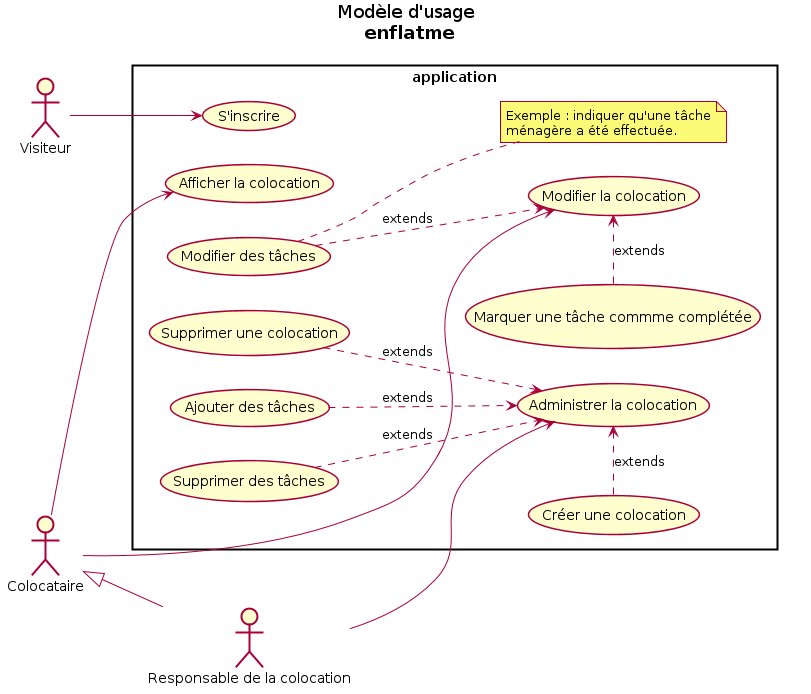
\includegraphics[scale=0.6]{../casUtilisation/casUtilisation.png}
		\caption{\label{fig:diagCasUtil}Diagramme des cas d'utilisation}
	\end{figure}
\end{center}
			\subsection{Division du travail en événement métier}
				\paragraph{Permettre le changement de colocation\\}
Il est possible dans la vie d'un utilisateur de déménager, il est donc nécessaire de lui permettre de changer ou quitter sa colocation pour, s'il le souhaite, en rejoindre une autre.

\paragraph{Être agréable à utiliser\\}
Pour que notre produit ait un réel succès, il est nécessaire que l'utilisateur n'apprécie pas le produit uniquement pour le service  qu'il propose. Il faut qu'il apprécie et aime l'utiliser ; il s'agit donc de s'inspirer des nombreux services populaires actuellement comme les réseaux sociaux.

\paragraph{Afficher clairement la gestion des tâches\\}
Notre produit est destiné à rendre plus facile la gestion d'une colocation et à servir de support pour prévenir les problèmes. Ainsi, il faut permettre aux utilisateurs d'interpréter facilement et de manière compréhensible leurs propres données.

		\section{Portée du Produit}
			\subsection{Modèle d'usage}
			\subsection{Description des cas d'utilisation}

		\section{Portée fonctionnelles}

	\chapter{Exigences non fonctionnelles}
		\section{Ergonomie et convivialité du produit}
			\subsection{L'interface}
L'application utilisera un design dit \textit{flat}, c'est-à-dire à posséder une interface avec des formes simples et nettes (pas de bords arrondis), sans ombres et sans dégradés. L'interface devra être uniforme entre l'application web et l'application mobile Android. L'application devra posséder une mascotte, qui reste encore à définir, qui aura vocation d'accompagner l'utilisateur dans la prise en main de l'application. Celle-ci sera présente et possédera une personnalité bien définie.\\

Les interactions avec l'interface doivent être rapides : l'interface doit être réactive et le nombre de gestes pour réaliser des actions doit être minimal.

\subsection{Le style du produit}
Le public doit correspondre aux interfaces que les jeunes ont l'habitude d'utiliser en ce moment, on pense particulièrement aux réseaux sociaux. L'application devra être colorée et être perçue comme moderne par nos utilisateurs.

		\section{Facilité d'utilisation et facteurs humains}
			\subsection{Facilité d'utilisation}
La prise en main de l'application doit se faire rapidement. C'est pourquoi on utilisera dès que possible des petits didacticiels pour montrer comment l'interface doit être utilisée. Pour ceci on pourra s'aider de notre mascotte où d'écrans de présentation. L'utilisateur doit pouvoir mémoriser facilement l'interface, c'est pourquoi on essaiera d'uniformiser celle-ci au maximum entre les différentes fonctionnalités.

\subsection{Personnalisation et internationalisation}
Notre application sera utilisable en Français et utilisera l'Euro comme monnaie. Il n'est pas prévu de proposer d'autres langues et d'autres monnaies dans un premier temps.

\subsection{Facilité d'apprentissage}
L'apprentissage de l'utilisation de l'application doit être immédiat pour éviter de perdre des utilisateurs rebutés par une interface trop complexe à comprendre.

\subsection{Facilité de compréhension et politesse}
L'application utilisera beaucoup d'icônes et aura un ton proche de l'utilisateur qui correspond à la culture des jeunes. Les messages pourront être ironiques et taquins dans des situations non critiques.

\subsection{Exigences d'accessibilité}
Aucune exigence particulière concernant les handicaps. Il est nécessaire de s'assurer que les éléments de l'interface ne soient pas trop petits pour pouvoir être touchés sur un mobile sans risque d'erreur.

		\section{Fonctionnement du produit}
			\subsection{Rapidité d'exécution et temps de latence}
La transition entre les écrans devra être la plus rapide possible. Pour l'application mobile, lorsque l'utilisateur n'est pas connecté au réseau Internet on mettra en cache les données qu'il souhaite envoyer et consulter. Celles-ci seront alors récupérées la prochaine fois qu'il sera en ligne.

\subsection{Exigences critiques de sécurité}
L'utilisation du produit n'entrainera pas un risque de sécurité particulier.

		
		% \section{Adéquation du produit avec son environnement}
		% 	\subsection{Environnement physique prévu}
Le site web sera utilisé dans un lieu calme, sur un ordinateur fixe ou portable où l'utilisateur pourra facilement se concentrer sur ce qu'il a à accomplir. Les utilisations de l'application mobile doivent pouvoir s'effectuer rapidement et ont pour vocation d'être courtes. Il est préférable d'inciter l'utilisateur à effectuer des tâches longues ou non adaptées pour le mobile sur le site web. On privilégiera l'application mobile pour des vérifications ou de légères mises à jour de statuts.

\subsection{Environnement technologique prévu}
Le site web doit être compatible avec tous les navigateurs (y compris Internet Explorer) pour les versions sorties il y a moins de 2 ans. L'application mobile doit être utilisable sur tous les téléphones Android pour une version supérieure à 4.

\subsection{Applications partenaires}
Nous ne souhaitons pas d'interactions avec des plate-formes extérieures, en particulier les réseaux sociaux.
\end{document}